\chapter{Modelare si proiectare}

\section{Cazurile utilizatorului si diagrame}
\label{sec:ch3sec1}
 \par Exista un sigur tip de utilizator care poate avea interactiune cu aplicatia, pe viitor se poate dezvolta inca un tip de user acesta avand scopul de a administra tabela cu filme. Fiecare utilizator are un nume unic si o parola pentru a se conecta la aplicatie, acolo unde el poate sa: caute filme, sa isi creeze propia lui lista cu filme, sa dea nota la un film sau sa vada detalii despre un film acolo unde sunt prezente si recomandari pentru filmul respectiv.
		\begin{figure}[htbp]
			\centerline{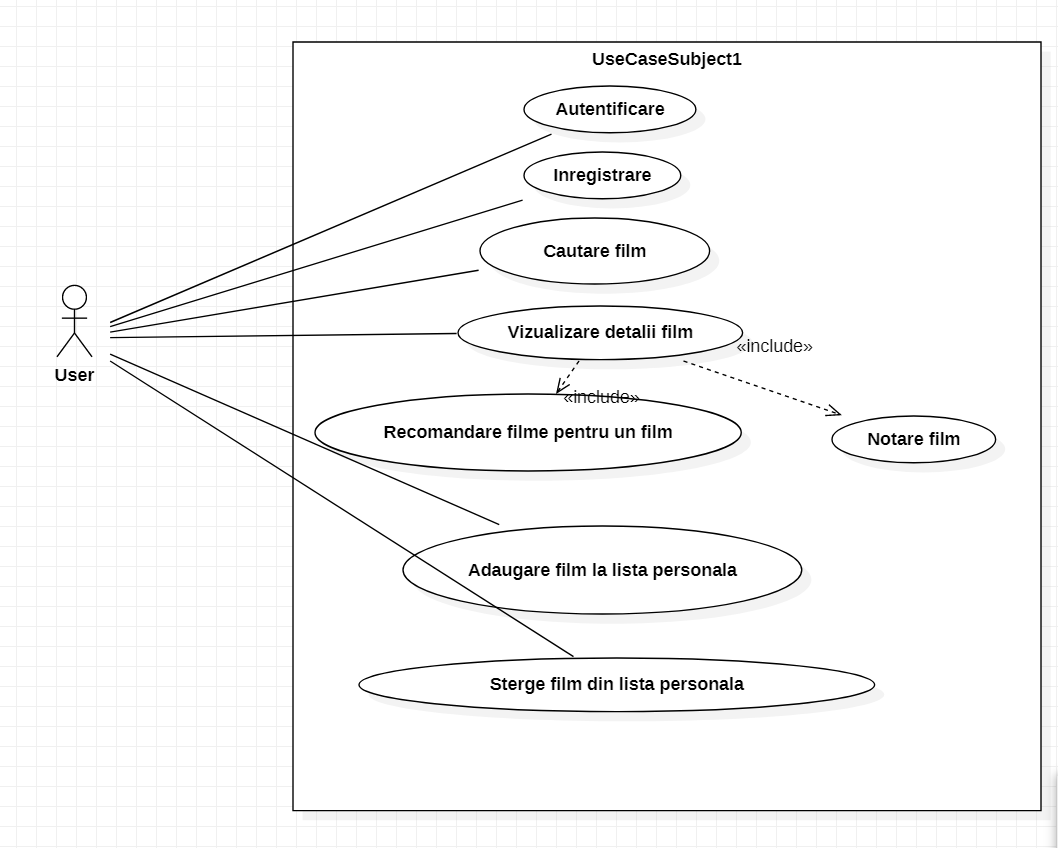
\includegraphics[width=13cm, height=10cm]{figures/use case.png}}
			\caption{Diagrama de cazuri}
			\label{fig}
		\end{figure}
\newline
\newline
\par \textbf{Figura 1}: Diagrama secventiala inregistrare
		\begin{figure}[htbp]
			\centerline{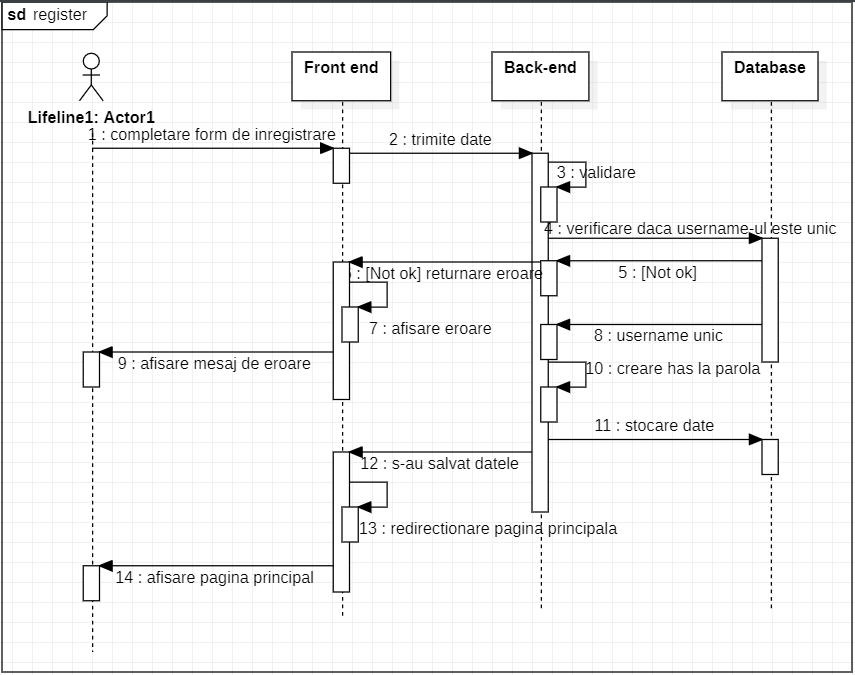
\includegraphics[width=13cm, height=8cm]{figures/sec register.png}}
			\caption{Diagrama secventiala pentru inregistrare}
			\label{fig}
		\end{figure}

\par \textbf{Figura 2}: Diagrama secventiala autentificare
		\begin{figure}[htbp]
			\centerline{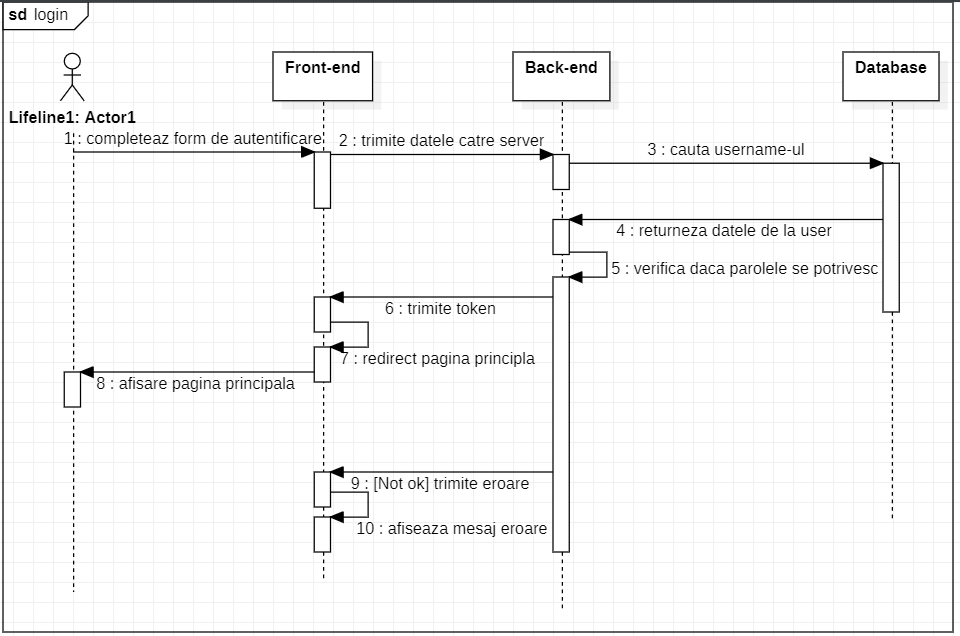
\includegraphics[width=13cm, height=8cm]{figures/login diagrma secventiala.png}}
			\caption{Diagrama secventiala pentru autentificare}
			\label{fig}
		\end{figure}
\newline
\newline
\newline
\newline
\newline
\par \textbf{Figura 3}: Diagrama secventiala adaugare film la lista personala
		\begin{figure}[!h]
			\centerline{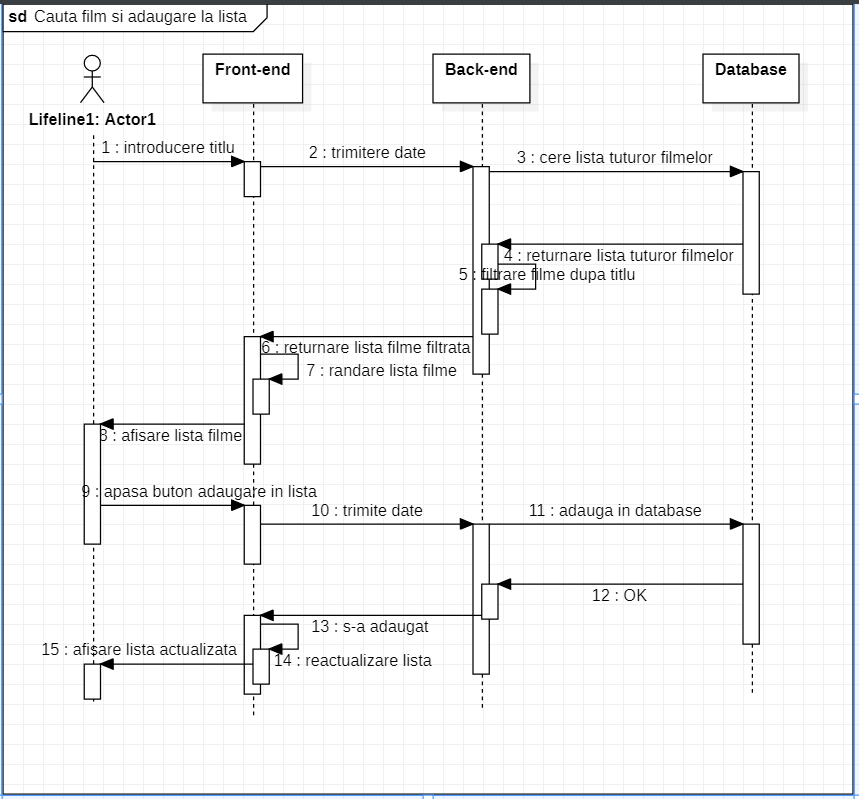
\includegraphics[width=14cm, height=10cm]{figures/cauta si adauga.png}}
			\caption{Diagrama secventiala adaugare film la lista}
			\label{fig}
		\end{figure}

\par \textbf{Figura 4}: Diagrama secventiala adaugare film la lista personala
		\begin{figure}[!h]
			\centerline{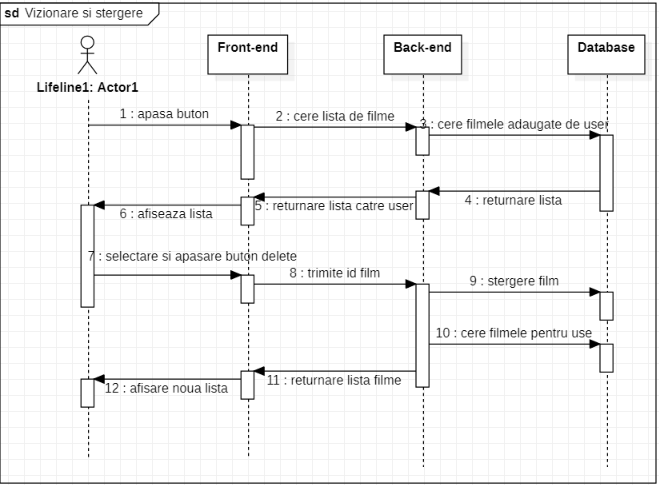
\includegraphics[width=14cm, height=10cm]{figures/fig.png}}
			\caption{Diagrama secventiala adaugare film la lista}
			\label{fig}
		\end{figure}

\par \textbf{Figura 5}: Acordare rating
		\begin{figure}[!h]
			\centerline{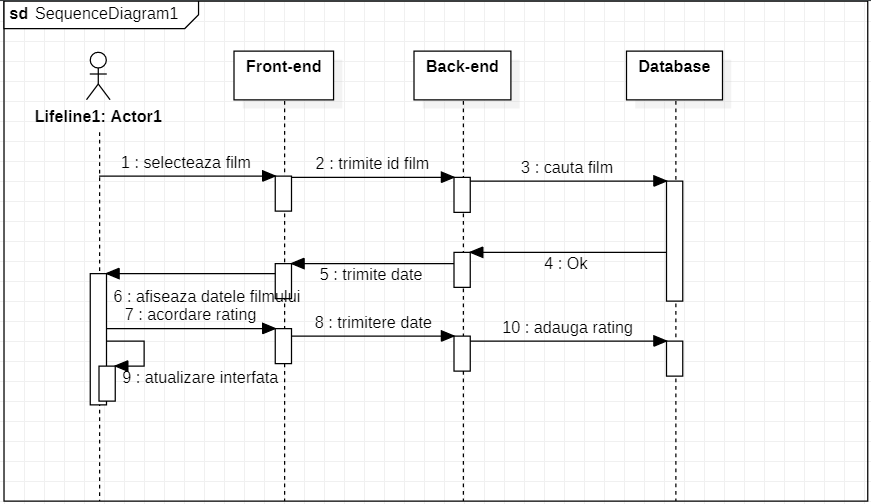
\includegraphics[width=14cm, height=10cm]{figures/acordare rating.png}}
			\caption{Diagrama secventiala adaugare film la lista}
			\label{fig}
		\end{figure}

\par \textbf{Figura 6}: Recomandare filme pentru un film
		\begin{figure}[!h]
			\centerline{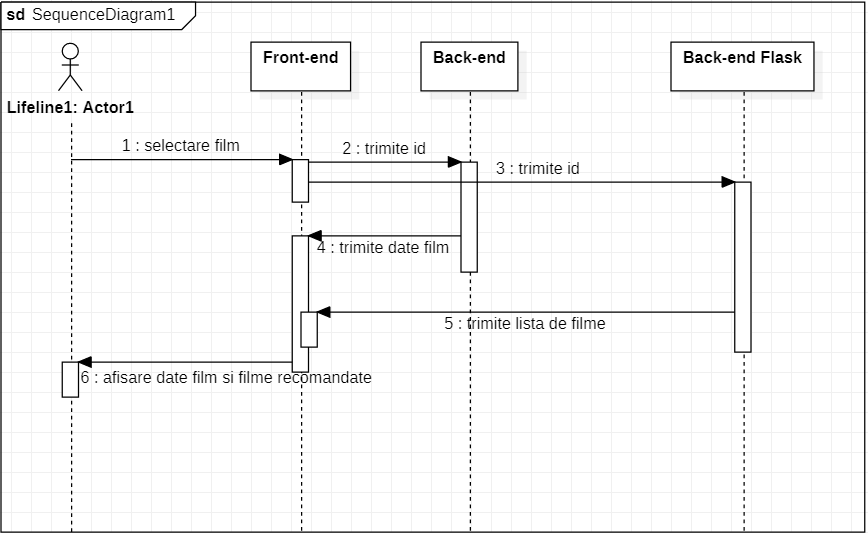
\includegraphics[width=14cm, height=10cm]{figures/recomandarea de filme.png}}
			\caption{Diagrama secventiala adaugare film la lista}
			\label{fig}
		\end{figure}

\section{Utilizarea aplicatiei}
\label{sec:ch3sec2}
\par Când utilizatorul aceseaza siteul acesta este redirectionat catre pagina de autentificare, daca acesta nu are cont poate apasa pe butonul Create account si v-a fi redirectionat către o pagina care contine un formular de înregistrare. După ce toate datele au fost comletate si înregistrarea a fost făcută cu succes acesta v-a fi redirectionat inpoi către pagina de autentificare, unde se poate autentifica cu noile credențiale.
\par După autentificare, utilizatorul este redirectionat către pagina principală unde in dreapta are un meniu de navigare si in centrul paginii o bara de căutare. Pe pagina principală utilizatorul poate să isi caute filme, după introducerea unui titlu si apasarea butonului de căutare i se vor afișa o lista cu toate filmele ce conțin in titlu șirul de caractere introduse de utilizator. Pe aceasta pagina un film poate avea una sau două posibilități: să se vada detalii despre film sau sa fie adăugat la lista personală de filme.
\par Dacă se apasa pe butonul de Detalii la un film utilizatorul este redirectionat catre pagina unde se pot vedea mai detaliile unui film, cum ar fi: titlu, descriere, actorii care joaca in film, tara de origine a filmului, directorii filmului, genurile, scriitorii care au venit cu idei pentru film, rating-ul general al filmului care reprezinta media notelor date de ceilanti utilizatori si cel mai important lucru se poate vedea patru filme recomandate pentru filmul respectiv. Tot pe aceasta pagina se poate acorda o nota filmului infuentand de altfel si nota generala a filmului.
\par Daca se apasa pe butonul de adaugare la lista personala filmul v-a fi adaugat, iar butonul respectiv v-a disparea. Pentru a vedea aceasta lista din meniul din dreapta se poate naviga catre pagina in care se prezinta lista cu filme adaugate de utilizator. Aceste filme tot doua butoane: unul de stergere care sterge filmul din lista si acelasi buton de detalii ca pe pagina principala.

